\newpage
\changeindent{0cm}
\section{実験と考察}
\changeindent{2cm}

本章では,実験と考察について説明する.
本研究では, 人工知能を用いた漫画の内容理解のために,
まず自然言語処理を用いて漫画のキャラクタのセリフの感情を推定する.
その上で漫画のコマの画像情報を加えたマルチモーダルな推定手法について実験する.
そして, 実験結果からセリフの感情推定とマルチモーダル化の精度への影響について考察する.

\changeindent{0cm}
\subsection{実験に使用したデータ}
\changeindent{2cm}

実験には上野の 4 コマ漫画ストーリーデータセットを用いた. このデータセットには 7 種類の感情ラベル(ニュートラル, 驚愕, 喜楽, 恐怖, 悲哀, 憤怒, 嫌悪)と, アノテーション不備によるラベル不明 (以下, ``UNK" とする) の全 8 種類
が含まれている. 今回は ``UNK" のデータを除いた全 7 種類の感情ラベルが付いたデータのみを用いた. 表 \ref{table:data_ori} に各タッチのオリジナルデータに対する感情ラベルごとのデータ数を示す.

\changeindent{0cm}
\subsection{実験設定}
\changeindent{2cm}

データ数と解析の難しさの問題から, 本研究では 7 種類ある感情ラベルのうち,
喜楽のみを正例クラス, その他の感情ラベルをすべて負例クラスとした
2 クラスのセリフの感情推定を行った.

訓練用データは各タッチの前半 1 話から 5 話までのオリジナルのセリフと
シソーラスを用いたデータ拡張によって生成されたセリフを用いて, 学習時には $20\%$ を検証用データとした.
また, 評価用モデルは検証用データにおける正例の F 値が最大となるエポックでのパラメータを採用した.
評価用データは後半 6 話から 10 話におけるオリジナルのセリフのみを用いた. そして, 各タッチに対してモデルを作成し評価をした.
表 \ref{table:data_exp} に各実験で用いた正例と負例のデータ数を示す.



\begin{table}[!ht]
\begin{center}
\caption{オリジナルデータ数} %タイトルをつける
\label{table:data_ori} %ラベルをつけ図の参照を可能にする
\begin{tabular}{lccccc|l}
\hline
\multirow{2}{*}{感情ラベル} & \multirow{2}{*}{ギャグ} & \multirow{2}{*}{少女} & \multirow{2}{*}{少年} & \multirow{2}{*}{青年} & \multirow{2}{*}{萌え} & \multirow{2}{*}{合計} \\
                       &                      &                     &                     &                     &                     &                     \\ \hline
喜楽                     & 25                   & 77                  & 27                  & 33                  & 47                  & 209 (31.7\%)        \\ \hline
ニュートラル                 & 43                   & 8                   & 55                  & 33                  & 30                  & 169 (25.6\%)        \\
驚愕                     & 19                   & 16                  & 17                  & 29                  & 20                  & 101 (15.3\%)        \\
悲哀                     & 25                   & 12                  & 13                  & 16                  & 13                  & 79 (12.0\%)         \\
恐怖                     & 6                    & 11                  & 8                   & 8                   & 9                   & 42 (6.4\%)          \\
憤怒                     & 4                    & 5                   & 2                   & 7                   & 2                   & 20 (3.0\%)          \\
嫌悪                     & 2                    & 4                   & 3                   & 3                   & 4                   & 16 (2.4\%)          \\ \hline
UNK                    & 7                    & 3                   & 5                   & 2                   & 6                   & 23 (3.5\%)          \\ \hline
合計                     & 131                  & 136                 & 130                 & 131                 & 131                 & 659
\end{tabular}
\end{center}
\end{table}

\begin{table}[!ht]
\begin{center}
\caption{実験で用いたデータ数} %タイトルをつける
\label{table:data_exp} %ラベルをつけ図の参照を可能にする
\begin{tabular}{llccccc|l}
\hline
\multirow{2}{*}{}       & \multirow{2}{*}{感情ラベル} & \multirow{2}{*}{ギャグ} & \multirow{2}{*}{少女} & \multirow{2}{*}{少年} & \multirow{2}{*}{青年} & \multirow{2}{*}{萌え} & \multirow{2}{*}{合計} \\
                        &                        &                      &                     &                     &                     &                     &                     \\ \hline
\multirow{2}{*}{訓練用データ} & 喜楽                     & 1115                 & 2672                & 940                 & 999                 & 1766                & 7492 (37.1\%)       \\
                        & その他                    & 2766                 & 1396                & 3077                & 3146                & 2324                & 12709 (62.9\%)      \\ \hline
\multirow{2}{*}{評価用データ} & 喜楽                     & 10                   & 38                  & 12                  & 14                  & 22                  & 96 (29.5\%)         \\
                        & その他                    & 56                   & 29                  & 52                  & 51                  & 42                  & 230 (70.5\%)
\end{tabular}
\end{center}
\end{table}


\changeindent{0cm}
\subsection{実験 1 : セリフ 1 文のみを入力とする感情推定}
\changeindent{2cm}

実験 1 では, セリフ 1 文のみを入力とする感情推定を行った.
まず, セリフ 1 文を BERT に入力し 768 次元のセリフベクトルを得る.
それを識別器への入力として, ``喜楽" か ``その他" かを推定した.
識別器としては 3 層 MLP を用いた.

本研究では, 各実験において Image Embedding 層には illustration2vec の筆者らによって公開されている事前学習済みモデルを用いた. Text Embedding 層には 2 種類の事前学習済み BERT モデルを用いた.

\newpage

一つは, 京都大学が公開している日本語 Wikipedia より全 1800 万文を用いて事前学習させたモデル \cite{kyoto-bert} (以下, ``京大 BERT" と呼ぶ) , もう一つは hottolink 社が公開している大規模日本語 SNS コーパスを用いて事前学習させたモデル, hottoSNS-BERT \cite{hottoSNS-bert} を用いた. BERT モデルは最終層のみを fine-tuning した.

表 \ref{table:mlp_para} に 3 層 MLP で用いたパラメータ, そして表 \ref{table:ex_para} に学習で用いたパラメータを示す. 学習率は Optuna \cite{optuna_2019} によって最適なパラメータを探索した.
また, 多くのタッチにおいて, 正例は負例に対してデータ数が非常に少ない不均衡データを扱うことから, このまま学習すると上手く学習が進まないという問題がある. 本研究ではこの解決策として, 損失関数のクラス重みとして, 訓練用データの各ラベルのデータ数の逆数を正規化したものを用いた. これにより, 正例がより正確に学習されると期待される. 表 \ref{table:ex_class_weight} に損失関数におけるタッチごとのクラス重みを示す.

\begin{table}[!h]
\vspace{20mm}
\caption{各実験における MLP のパラメータ}
\label{table:mlp_para}
\centering
\scalebox{1.35}{
\begin{tabular}{c|cc}
\hline
パラメータ & 実験 1 & 実験 2 \\ \hline
入力層次元 & 768 & 4864 \\
隠れ層次元 & \multicolumn{2}{c}{30} \\
出力層次元 & \multicolumn{2}{c}{2} \\ \hline
活性化関数 & \multicolumn{2}{c}{tanh} \\ \hline
ドロップアウト率 & \multicolumn{2}{c}{0.5}
\end{tabular}
}
\end{table}

\newpage

\begin{table}[!h]
\vspace{10mm}
\caption{学習パラメータ}
\label{table:ex_para}
\centering
\scalebox{1.35}{
\begin{tabular}{c|c|l}
\hline
パラメータ  & \multicolumn{2}{c}{実験 $1・2$}           \\ \hline
エポック数  & \multicolumn{2}{c}{50}                 \\ \hline
バッチサイズ & \multicolumn{2}{c}{16}                 \\ \hline
損失関数   & \multicolumn{2}{c}{Cross Entropy Loss\footnotetext[1]{出力層では softmax}} \\ \hline
最適化手法  & \multicolumn{2}{c}{Adam}
\end{tabular}
}
\vspace{10mm}
\end{table}

\begin{table}[!h]
\vspace{10mm}
\caption{損失関数におけるクラス重み}
\label{table:ex_class_weight}
\centering
\scalebox{1.35}{
\begin{tabular}{c|l|l}
\hline
タッチ                          & \multicolumn{1}{c|}{正例} & \multicolumn{1}{c}{負例} \\ \hline
ギャグタッチ                       & 0.773                   & 0.227                  \\
少女漫画タッチ                      & 0.272                   & 0.728                  \\
\multicolumn{1}{l|}{少年漫画タッチ} & 0.831                   & 0.169                  \\
青年漫画タッチ                      & 0.824                   & 0.176                  \\
萌えタッチ                        & 0.594                   & 0.406
\end{tabular}
}
\end{table}

\newpage
\changeindent{0cm}
\subsection{実験 1 : 結果}
\changeindent{2cm}

表 \ref{table:result_1} に評価用データに対する実験 1 の結果を示す. 表 \ref{table:result_1} における P-Recall, P-F 値はそれぞれ正例の再現率, F 値を表し, Acc は全体の精度を表している. また, 5 タッチ総合の結果は各タッチの結果における混合行列の和から算出している.
本研究では, ベースラインは前述のように, 正例が負例に対してデータ数が
非常に少ない不均衡データであることから, すべての予測値が負例の場合を設定した.
図 \ref{fig:ex1_graph} に Text Embedding 層に hottoSNS-BERT を用いた場合のギャグタッチにおける学習曲線を示す. 左の図から Acc, 正例の F 値, loss を表し, 青線は訓練用データ, オレンジの線は検証用データを表す.

表 \ref{table:result_1} より, Acc に関してはどちらの BERT モデルを用いても
ベースラインを超えた. また, ほとんどの評価指標において京大 BERT よりも hottoSNS-BERT の方が優れた結果を示した. 図 \ref{fig:ex1_graph} において, 訓練用データと検証用データの学習曲線の推移が酷似しているのは, データの切り分け方に問題があると推測される. 前述のように, 4 コマ漫画ストーリーデータセットには現状, 同一のストーリーを原則的に 4 コマ目がオチとなる ``一般" と逆に 1 コマ目にオチを持ってきた ``出オチ" の 2 種類の構造のみからなっており, セリフやその感情ラベルに大きな差はない. つまり, 似たセリフデータが 2 つずつ存在している場合が多い. そのため, 検証用データをランダムにサンプリングしたことでデータの分布にも差が生まれず, 訓練用データと検証用データの学習曲線の推移が酷似したと考えられる.

\begin{figure}[!h]
  \vspace{5mm}
  \centering
  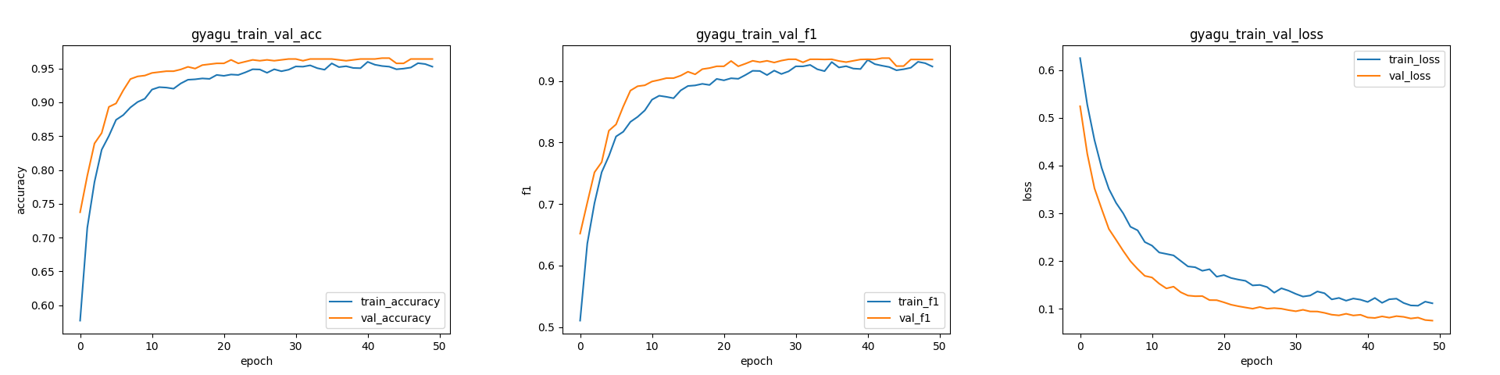
\includegraphics[width=1.0\hsize]{doc/figures/ex1_graph_hotto_gyagu.png}
  \caption{実験 1 における学習曲線の例}
  \label{fig:ex1_graph}
\end{figure}

\newpage
\begin{table}[!hb]
\vspace{15mm}
\begin{center}
\caption{評価用データに対する実験 1 の結果}
\label{table:result_1}
\scalebox{1.0}{
\begin{tabular}{lcccccc}
\hline
\multicolumn{1}{c}{\multirow{2}{*}{}} & \multicolumn{3}{c}{ギャグタッチ} & \multicolumn{3}{c}{少女漫画タッチ} \\
\multicolumn{1}{c}{} & Acc & P-Recall & P-F 値 & Acc & P-Recall & P-F 値 \\ \hline
京大 BERT & {\ul 0.818} & 0.200 & 0.250 & 0.612 & 0.711 & 0.675 \\
hottoSNS-BERT & {\ul 0.818} & 0.300 & {\ul 0.333} & {\ul 0.627} & 0.816 & {\ul 0.713} \\ \hline
ベースライン & \multicolumn{1}{l}{0.848} & - & - & 0.432 & - & - \\
 & \multicolumn{1}{l}{} & \multicolumn{1}{l}{} & \multicolumn{1}{l}{} & \multicolumn{1}{l}{} & \multicolumn{1}{l}{} & \multicolumn{1}{l}{} \\
 & \multicolumn{1}{l}{} & \multicolumn{1}{l}{} & \multicolumn{1}{l}{} & \multicolumn{1}{l}{} & \multicolumn{1}{l}{} & \multicolumn{1}{l}{} \\ \hline
\multicolumn{1}{c}{} & \multicolumn{3}{c}{少年漫画タッチ} & \multicolumn{3}{c}{青年漫画タッチ} \\
\multicolumn{1}{c}{} & Acc & P-Recall & P-F 値 & Acc & P-Recall & P-F 値 \\ \hline
京大 BERT & 0.766 & 0.083 & 0.118 & {\ul 0.862} & 0.500 & 0.609 \\
hottoSNS-BERT & {\ul 0.813} & 0.167 & {\ul 0.250} & 0.846 & 0.643 & {\ul 0.643} \\ \hline
ベースライン & 0.812 & - & - & 0.784 & - & - \\
 & \multicolumn{1}{l}{} & \multicolumn{1}{l}{} & \multicolumn{1}{l}{} & \multicolumn{1}{l}{} & \multicolumn{1}{l}{} & \multicolumn{1}{l}{} \\
 & \multicolumn{1}{l}{} & \multicolumn{1}{l}{} & \multicolumn{1}{l}{} & \multicolumn{1}{l}{} & \multicolumn{1}{l}{} & \multicolumn{1}{l}{} \\ \hline
 & \multicolumn{3}{c}{萌えタッチ} & \multicolumn{3}{c}{5 タッチ総合} \\
 & Acc & P-Recall & P-F 値 & Acc & P-Recall & P-F 値 \\ \hline
京大 BERT & 0.609 & 0.591 & 0.510 & 0.733 & 0.521 & 0.535 \\
hottoSNS-BERT & {\ul 0.688} & 0.500 & {\ul 0.524} & {\ul 0.758} & 0.583 & {\ul 0.586} \\ \hline
ベースライン & 0.656 & - & - & 0.705 & - & -
\end{tabular}
}
\end{center}
\end{table}

\newpage
\changeindent{0cm}
\subsection{実験 2 : マルチモーダルな感情推定の検討}
\changeindent{2cm}

実験 2 では, 提案手法に則って, マルチモーダルな感情推定の検討を行った.
実験 1 と同様に BERT から得た 768 次元のセリフベクトルと, 入力したセリフが含まれているコマ全体の画像を illustration2vec に入力して得た 4096 次元のコマベクトルを単純に結合させた 4864 次元のベクトルを識別器である 3 層 MLP に入力することでマルチモーダルな感情推定をした.

表 \ref{table:mlp_para} に 3 層 MLP で用いたパラメータ, そして表 \ref{table:ex_para} に学習で用いたパラメータを示す. その他の実験設定は実験 1 と同様にした.


\changeindent{0cm}
\subsection{実験 2 : 結果}
\changeindent{2cm}

表 \ref{table:result_2} に評価用データに対する実験 2 の結果を示す. また, 図 \ref{fig:ex1_graph} に Text Embedding 層に hottoSNS-BERT を用いた場合のギャグタッチにおける学習曲線を示す. 実験 1 と同様に左の図から Acc, 正例の F 値, loss を表し, 青線は訓練用データ, オレンジの線は検証用データを表す. また, 5 タッチ総合の結果は各タッチの結果における混合行列の和から算出している.

表 \ref{table:result_2} より, Acc に関してはどちらの BERT モデルを用いても
同様にベースラインを超えた. ほとんどの評価指標において京大 BERT よりも hottoSNS-BERT の方が上回り, 実験 1 および 実験 2 を通してそれぞれ最も高い値を示したことから, 京大 BERT よりも hottoSNS-BERT の方が漫画のセリフの分散表現の獲得手法として有効であると定量的に確認した. そして, 5 タッチ総合の結果より実験 1 よりも正例の識別率も向上したことから, マルチモーダルな感情推定の有効性を定量的に確認した. 図 \ref{fig:ex2_graph} において, 訓練用データと検証用データの学習曲線の推移が実験 1 の学習曲線より急勾配で早期に収束している. これは単純に識別器への入力次元数が増えたことに起因すると考えられる. そして, 多くのタッチにおいて実験 1 ではほとんど識別できていなかった正例データが識別できていたことを確認した.
図 \ref{fig:multimodal_add_seikai} にこれらの正例データを示す. 図 \ref{fig:multimodal_add_seikai} のオレンジの枠で囲われたセリフより, 文字だけでは人間の目で見ても判断が難しいが, 画像情報 (発話者の顔の表情) を加味することで喜楽寄りのセリフであると理解できるデータであることが分かる.

\newpage
\begin{table}[!ht]
\vspace{15mm}
\begin{center}
\caption{評価用データに対する実験 2 の結果}
\label{table:result_2}
\scalebox{1.0}{
\begin{tabular}{lcccccc}
\hline
\multicolumn{1}{c}{\multirow{2}{*}{}} & \multicolumn{3}{c}{ギャグタッチ} & \multicolumn{3}{c}{少女漫画タッチ} \\
\multicolumn{1}{c}{} & Acc & P-Recall & P-F 値 & Acc & P-Recall & P-F 値 \\ \hline
京大 BERT & 0.773 & 0.200 & 0.211 & 0.687 & 0.763 & 0.734 \\
hottoSNS-BERT & {\ul 0.818} & 0.400 & {\ul 0.400} & {\ul 0.761} & 0.816 & {\ul 0.795} \\ \hline
ベースライン & \multicolumn{1}{l}{0.848} & - & - & 0.432 & - & - \\
 & \multicolumn{1}{l}{} & \multicolumn{1}{l}{} & \multicolumn{1}{l}{} & \multicolumn{1}{l}{} & \multicolumn{1}{l}{} & \multicolumn{1}{l}{} \\
 & \multicolumn{1}{l}{} & \multicolumn{1}{l}{} & \multicolumn{1}{l}{} & \multicolumn{1}{l}{} & \multicolumn{1}{l}{} & \multicolumn{1}{l}{} \\ \hline
\multicolumn{1}{c}{} & \multicolumn{3}{c}{少年漫画タッチ} & \multicolumn{3}{c}{青年漫画タッチ} \\
\multicolumn{1}{c}{} & Acc & P-Recall & P-F 値 & Acc & P-Recall & P-F 値 \\ \hline
京大 BERT & 0.703 & 0.417 & 0.345 & 0.769 & 0.643 & {\ul 0.545} \\
hottoSNS-BERT & {\ul 0.781} & 0.500 & {\ul 0.462} & {\ul 0.815} & 0.500 & 0.538 \\ \hline
ベースライン & 0.812 & - & - & 0.784 & - & - \\
 & \multicolumn{1}{l}{} & \multicolumn{1}{l}{} & \multicolumn{1}{l}{} & \multicolumn{1}{l}{} & \multicolumn{1}{l}{} & \multicolumn{1}{l}{} \\
 & \multicolumn{1}{l}{} & \multicolumn{1}{l}{} & \multicolumn{1}{l}{} & \multicolumn{1}{l}{} & \multicolumn{1}{l}{} & \multicolumn{1}{l}{} \\ \hline
 & \multicolumn{3}{c}{萌えタッチ} & \multicolumn{3}{c}{5 タッチ総合} \\
 & Acc & P-Recall & P-F 値 & Acc & P-Recall & P-F 値 \\ \hline
京大 BERT & 0.641 & 0.500 & 0.489 & 0.715 & 0.583 & 0.546 \\
hottoSNS-BERT & {\ul 0.703} & 0.545 & {\ul 0.558} & {\ul 0.776} & 0.625 & {\ul 0.622} \\ \hline
ベースライン & 0.656 & - & - & 0.705 & - & -
\end{tabular}
}
\end{center}
\vspace{10mm}
\end{table}

\newpage

\begin{figure}[!h]
  \centering
  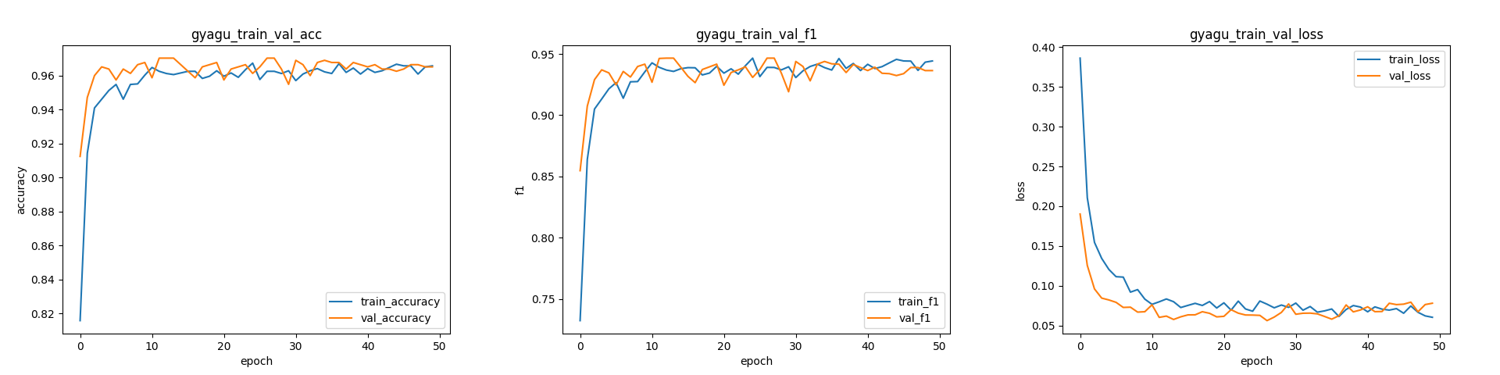
\includegraphics[width=1.0\hsize]{doc/figures/ex2_graph_hotto_gyagu.png}
  \caption{実験 2 における学習曲線の例}
  \label{fig:ex2_graph}
\end{figure}

\begin{figure}[!h]
  \vspace{15mm}
  \centering
  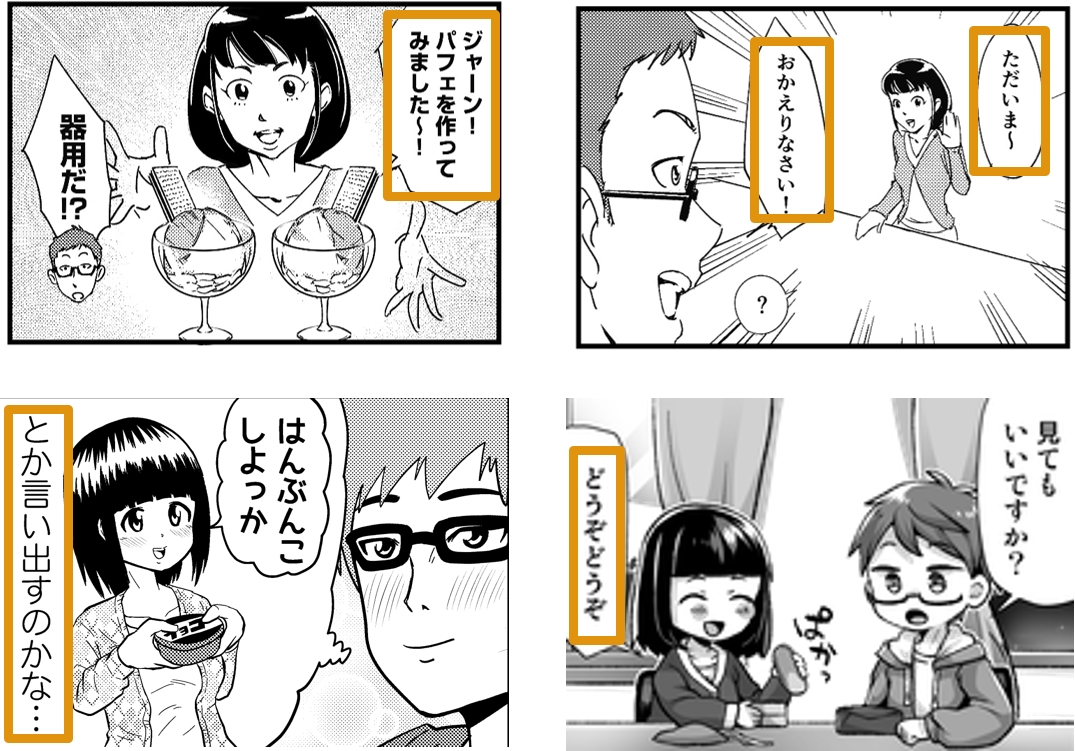
\includegraphics[width=0.8\hsize]{doc/figures/multimodal_add_seikai.png}
  \caption{マルチモーダル化の精度への影響}
  \label{fig:multimodal_add_seikai}
\end{figure}

\newpage
\changeindent{0cm}
\subsection{考察}
\changeindent{2cm}

\changeindent{0cm}
\subsubsection{BERT モデルの合理性とシソーラスを用いたデータ拡張の問題}
\changeindent{2cm}

実験結果から, 定量的に京大 BERT よりも hottoSNS-BERT の方が漫画のセリフの分散表現の獲得手法として優れていることが示せた. ここで, 別の視点から京大 BERT と hottoSNS-BERT のどちらがより合理的な分散表現を得られているかについて考察する.

図 \ref{fig:cos_bert} にシソーラスを用いたデータ拡張によって生成されたセリフとそれぞれに対応するオリジナルのセリフとのコサイン類似度を, 京大 BERT と hottoSNS-BERT を用いて計算したヒストグラムを示す. 横軸はコサイン類似度, 縦軸は区間内のデータ数を表している. また, 青色が hottoSNS-BERT, オレンジ色が京大 BERT を表す. ここで, コサイン類似度とは 2 本のベクトルがどれくらい同じ向きを向いているのかを表す指標であり, $-1$ から $1$ までの値を取る. まったく同じ文章同士であればコサイン類似度は $1$ であり, 似た文章であるほど $1$ に近い値を示す.

\begin{figure}[!h]
  \centering
  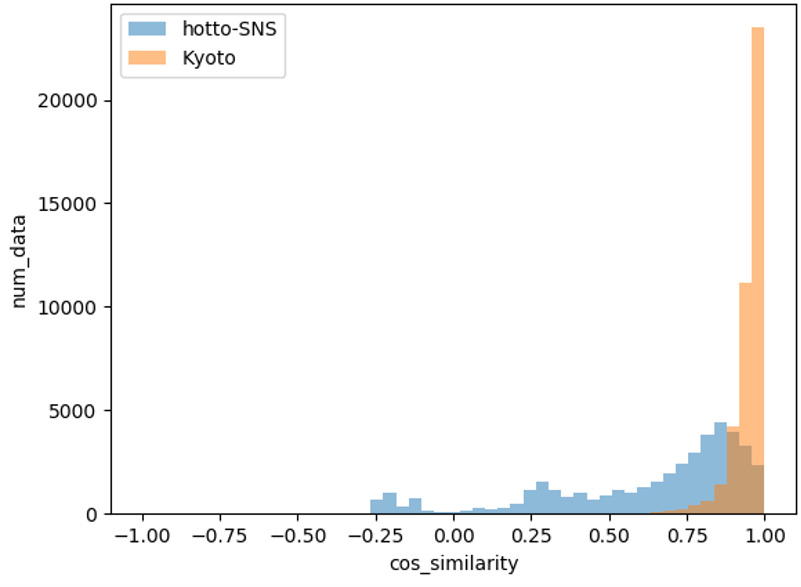
\includegraphics[width=0.8\hsize]{doc/figures/cos_bert.png}
  \caption{拡張されたセリフと対応するオリジナルのセリフとのコサイン類似度}
  \label{fig:cos_bert}
\end{figure}

\newpage
図 \ref{fig:cos_bert} より, 一見して京大 BERT の方がコサイン類似度が高い区間に集まっていることから, 優れているように考えられる. しかし, これはデータ拡張の手法に大きな問題が無いという前提でのみ成立する. 本研究におけるシソーラスを用いたデータ拡張には, 文法的意味に齟齬が発生しているという問題がある. 例としては, 意味は通じるが形容詞であったものが名詞に置き換わっていたり, 文法的に間違ったものも含まれていた.

表 \ref{table:sogo} にシソーラスを用いたデータ拡張によって文法的齟齬が生じているデータに対するコサイン類似度を, 京大 BERT と hottoSNS-BERT から出力されたセリフベクトルを用いて計算した結果を示す. 表 \ref{table:sogo} より, 人間の目で見てもオリジナルのセリフから意味が遠いように思えたり, 文法的齟齬があるセリフに対して, 京大 BERT は高いコサイン類似度を示している一方で, hottoSNS-BERT は $0.8$ 付近にある一番大きな山には属さず, マイナスの値を取っている. このことから, 定性的にも京大 BERT よりも hottoSNS-BERT の方が漫画のセリフの分散表現の獲得手法として優れていると推測できる.

\begin{table}[!h]
\vspace{20mm}
\caption{シソーラスを用いたデータ拡張による文法的齟齬}
\label{table:sogo}
\centering
\scalebox{1.0}{
\begin{tabular}{ll|cc}
\multicolumn{1}{c}{オリジナルのセリフ} & \multicolumn{1}{c|}{拡張後のセリフ} & 京大 BERT & hottoSNS-BERT \\ \hline
去年は私が着たやつ & 去年は私が着た若者 & 0.97 & -0.19 \\ \hline
そうですか & 正しくですか & 0.89 & -0.19 \\ \hline
\begin{tabular}[c]{@{}l@{}}僕はいいですけど、\\ 気をつけてくださいね\end{tabular} & \begin{tabular}[c]{@{}l@{}}僕はグーですけど、\\ 気をつけてくださいね\end{tabular} & 0.96 & -0.16 \\ \hline
 & \begin{tabular}[c]{@{}l@{}}僕はいいですけど、\\ 真性をつけてくださいね\end{tabular} & 0.94 & 0.25
\end{tabular}
}
\vspace{10mm}
\end{table}

\newpage

また, シソーラスを用いたデータ拡張による文法的齟齬に関する問題の解決策としては, 拡張
されたセリフの分散表現とそれぞれに対応するオリジナルのセリフの分散表現とのコサイン類似度から閾値未満のデータを除外したり, 拡張する品詞を限定するといったことが考えられる.

そして, hottoSNS-BERT には特殊なトークンとして ``$<$mention$>$" が存在する. これは, 事前学習で用いた日本語 SNS コーパスの中で, リプライ (返信) に該当するデータの文頭に付与されるトークンである. 図 \ref{fig:mention} に $<$mention$>$ トークンの例を示す. 人手によってアノテートする必要はあるものの, このトークンを付与することによって, より会話の流れを汲んだ学習が可能になると考えられる. 応用例としては, 会話破綻の検出や人工知能を用いた会話の自動生成などが考えられる.

\begin{figure}[!h]
  \vspace{20mm}
  \centering
  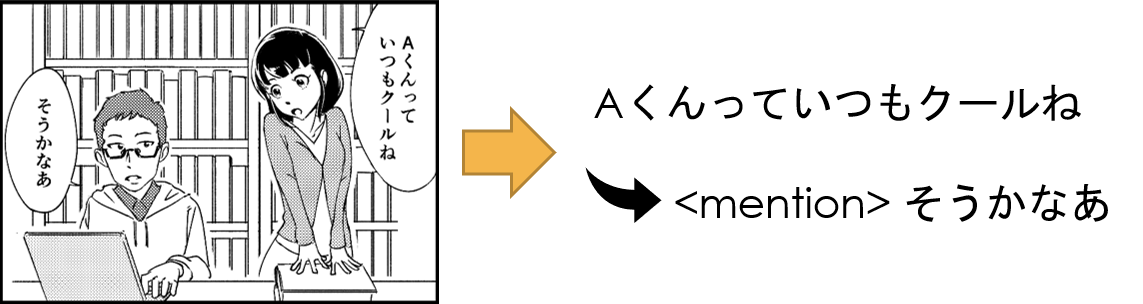
\includegraphics[width=1.0\hsize]{doc/figures/mention.png}
  \caption{$<$mention$>$ トークンの概要}
  \label{fig:mention}
\end{figure}

\newpage
\changeindent{0cm}
\subsubsection{illustration2vec モデルの合理性について}
\changeindent{2cm}

次に, 本研究で用いた illustration2vec モデルの合理性について考察する. 実験結果よりマルチモーダルな感情推定の有効性を定量的に確認した. しかし, どのような情報が取れているのかについては不明瞭である. そこで, t-SNE (t-distribution Stochastic Neighbor Embedding) \cite{vanDerMaaten2008} を用いてコマベクトルを 2 次元に圧縮し, 可視化した. 図 \ref{fig:koma_tsne} にその結果を示す.

\begin{figure}[!h]
  \vspace{5mm}
  \centering
  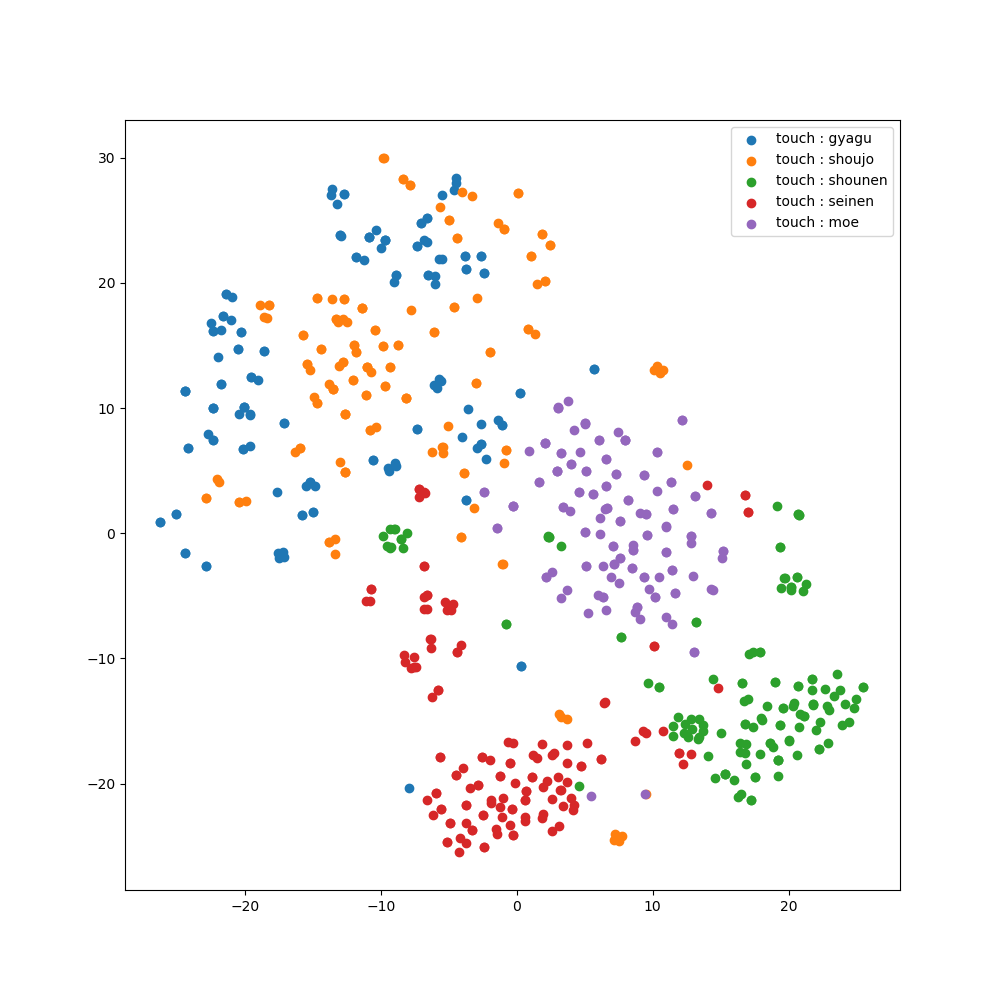
\includegraphics[width=0.9\hsize]{doc/figures/koma_tsne.png}
  \caption{コマベクトルの t-SNE による次元圧縮結果}
  \label{fig:koma_tsne}
\end{figure}

\newpage
図 \ref{fig:koma_tsne} より, 少年漫画タッチ, 青年漫画タッチ, 萌えタッチではタッチごとに大きくまとまっていることが確認できる. ギャグタッチと少女漫画タッチについてもいくつかのまとまりが確認できることから, illustration2vec によって得られたコマベクトルはタッチの情報をうまく反映していると言える.

また, 本研究では illustration2vec をコマベクトルを得るためのエンコーダとしてのみ用いたが, illustration2vec では多クラスのラベル予測が可能である. 図 \ref{fig:i2v_tag} にその例を示す. ラベル予測の結果はラベル名とその確率で与えられる. 図 \ref{fig:i2v_tag} より, ``モノクローム", ``1 人の女の子", ``1 人の男の子", ``眼鏡", ``ショートヘア", といったようにコマ画像に含まれるものをよくとらえていることが分かる. このことから, より精度の高いマルチモーダルな感情推定を行うためには illustration2vec モデルの fine-tuning が有効であると考えられる. illustration2vec のラベルには ``smile", ``angry", ``surprised", といった感情に関係するものも含まれている. よって, 1 コマの中にどのような感情が含まれているか, といったメタ情報を付加し学習させることによって, より合理的なコマベクトルを得られると考えられる. また, 漫画では一般に読者にキャラクタの感情をより分かりやすく説明するための方法として, オノマトペやスクリーントーンの活用, 効果線, 吹き出しの形状などが挙げられる. 実際に, 上野らの研究 \cite{ueno-emotion2016} によってキャラクタ間の感情をキャラクタの表情と吹き出しの形状から理解することが有用である可能性が高いことが示されていることから, コマ画像の特徴的要素を付加したマルチモーダルな感情推定についても有用であると考えられる.

\begin{figure}[!h]
  \vspace{10mm}
  \centering
  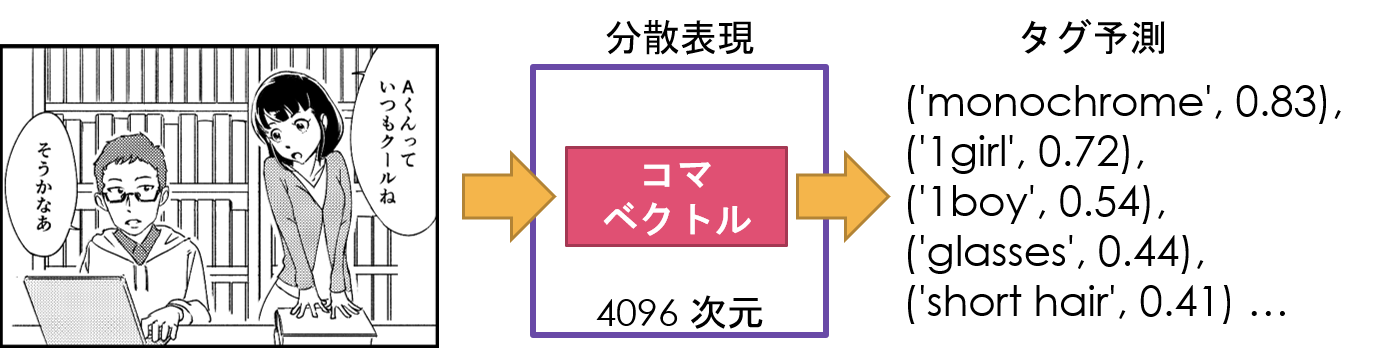
\includegraphics[width=0.9\hsize]{doc/figures/illustration2vec_tag.png}
  \caption{illustration2vec による多クラスのラベル予測例}
  \label{fig:i2v_tag}
\end{figure}

\newpage

\changeindent{0cm}
\subsubsection{マルチモーダル特徴量の結合方法の問題}
\changeindent{2cm}

本研究では, セリフベクトルとコマベクトルを単純に結合させることでマルチモーダルな感情推定を行った. しかし, それが最も良い方法であるという確証はない. この問題の解決策として, Differentiable Architecture Search (DARTS) \cite{DBLP:journals/corr/abs-1806-09055} をはじめとしたニューラルネットワークの設計を自動化する手法, Neural Architecture Search (NAS) を用いて最適なマルチモーダル特徴量の結合構造を探索することなどが考えられる. こちらの適用については今後の課題とする.

\changeindent{0cm}
\subsection{補足 : 人手による新たなセリフデータの作成}
\changeindent{2cm}

本研究で行った実験には使用しなかったが, 4 コマ漫画ストーリーデータセットの問題点であるデータの少なさを改善するために, 人手による新たなセリフデータの作成を現在行っている. 以下にセリフデータの作成手順を示す.

\begin{enumerate}
  \item データを拡張する対象のタッチを萌えタッチのみとし, また一部の 4 コマを除外する.
  \item 使用するデータのセリフの吹き出しを白抜きし, 順番にセリフに対して固有の id を与える.
  \item id に加え, 発話者の情報などをまとめた csv ファイルを用意し, アノテータに各 id に対応するセリフとその感情ラベルを付与してもらう.
\end{enumerate}

また, 4 コマ漫画ストーリーデータセットの大きな特徴である ``作者によるセリフの感情アノテーション" を担保するために以下の条件を付け加えた.

\begin{itemize}
  \item 1 つの 4 コマ内での物語の一貫性を保つ.
  \item 登場人物の名前を独自に付ける. \\ (オリジナルデータでは ``A くん", ``B さん" といった抽象的な名前が付けられている.)
\end{itemize}

\newpage
現状は自分を含めた 2 人分のアノテートが完了している. これらを拡張萌えタッチ A, 拡張萌えタッチ B とする. 図 \ref{fig:shironuki} に白抜きされた 4 コマ画像の例, 表 \ref{table:aug_data} に, 図 \ref{fig:shironuki} に対応する拡張萌えタッチ A のデータ例を示す.

\begin{figure}[!h]
  \vspace{1mm}
  \centering
  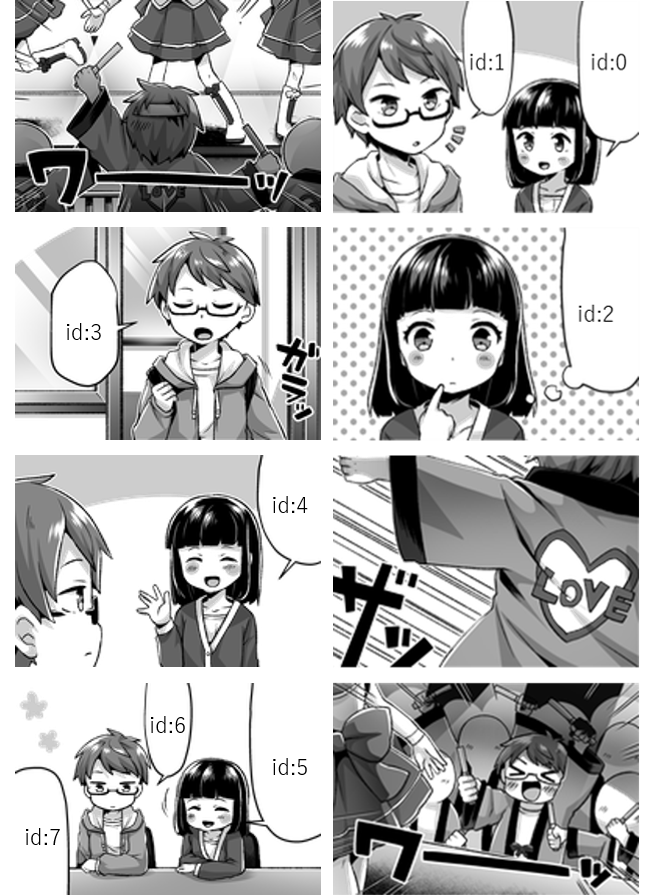
\includegraphics[width=0.4\hsize]{doc/figures/shironuki.png}
  \caption{アノテーションのための白抜き 4 コマ画像の例}
  \label{fig:shironuki}
\end{figure}

\begin{table}[!h]
\vspace{5mm}
\caption{アノテートされたセリフと感情ラベルの例}
\label{table:aug_data}
\centering
\scalebox{0.8}{
\begin{tabular}{c|l|c}
id & \multicolumn{1}{c|}{セリフ (拡張萌えタッチ A)} & 感情ラベル  \\ \hline
0  & 小池君 今週末の予定は?             & 喜楽     \\
1  & 研究の進捗を生みますよ              & ニュートラル \\
2  & 本当かなぁ?                      & ニュートラル \\
3  & 百合子さん こんにちは              & ニュートラル \\
4  & 週末は随分と楽しんだみたいね           & 嫌悪     \\
5  & 研究しないと留年するよ?             & 悲哀     \\
6  & 分かってはいるのですが・・・           & 悲哀     \\
7  & 一緒に卒業しようね!               & 喜楽
\end{tabular}
}
\vspace{1mm}
\end{table}

\newpage
また, 表 \ref{table:data_moe_aug} に拡張萌えタッチ A, 拡張萌えタッチ B それぞれの感情ラベルごとのデータ数を示す. アノテートミスのあるデータを除いた, セリフの感情ラベルが一致した割合は $44.4 \%$ であった. この結果と表 \ref{table:data_moe_aug} から, この手法を用いることで多様な 4 コマ漫画ストーリーデータセットの拡張が可能であると言える. これらのデータを活用することでより汎化性能の高いモデルの生成が期待できる.


\begin{table}[!h]
\vspace{20mm}
\begin{center}
\caption{アノテートされたデータ数} %タイトルをつける
\label{table:data_moe_aug} %ラベルをつけ図の参照を可能にする
\begin{tabular}{lcc}
\hline
\multirow{2}{*}{感情ラベル} & \multirow{2}{*}{拡張萌えタッチ A} & \multirow{2}{*}{拡張萌えタッチ B} \\
 &  &  \\ \hline
喜楽 & 33 & 27 \\ \hline
ニュートラル & 26 & 33 \\
驚愕 & 11 & 11 \\
悲哀 & 18 & 5 \\
恐怖 & 1 & 9 \\
憤怒 & 3 & 11 \\
嫌悪 & 7 & 1 \\ \hline
アノテートミス & 0 & 2 \\ \hline
合計 & 99 & 99
\end{tabular}
\end{center}
\vspace{10mm}
\end{table}

% \begin{table}[!h]
% \vspace{20mm}
% \begin{center}
% \caption{拡張されたデータ数} %タイトルをつける
% \label{table:data_moe_aug} %ラベルをつけ図の参照を可能にする
% \begin{tabular}{lcc}
% \hline
% \multirow{2}{*}{感情ラベル} & \multirow{2}{*}{拡張萌えタッチ A} & \multirow{2}{*}{拡張萌えタッチ B} \\
%  &  &  \\ \hline
% 喜楽 & 33 & 27 \\ \hline
% ニュートラル & 26 & 33 \\
% 驚愕 & 11 & 13 \\
% 悲哀 & 18 & 5 \\
% 恐怖 & 1 & 9 \\
% 憤怒 & 3 & 11 \\
% 嫌悪 & 7 & 1 \\ \hline
% 合計 & 99 & 99
% \end{tabular}
% \end{center}
% \vspace{10mm}
% \end{table}
